\section{Physics Theory}
\label{sec:PhysicsTheory}

\subsection{Laminated Glass Model}

%Picture of Laminated Glass
%Measurements of the plies and inter-layer

Laminated glass is a sandwich structure of two brittle glass plies and an adhered polymer inter-layer (or inter-face) in between. The bonding between the glass and the inter-layer is without physical adhesive \cite{Sam19}. Secondary laminated glass consists of two such laminates, separated by a layer of air.

\bigbreak
Advantageous properties of laminated glass include a relatively high penetration resistance \cite{Xu14}, low weight \cite{Wu14} and the adherence of fractured glass fragments to the structure to reduce the risk of injuries\cite{Xu14, Che17, Flo98, Ji98}. Breakage of the inner ply significantly reduces strength and facilitates a full collapse of the glass \cite{Flo98}. An optional back layer (usually poly-carbonate (\texttt{PC}) \cite{Bra10, Mon04}) improves structural stability and additional energy absorption \cite{Bio10, Bra10}.

\bigbreak
The prediction of crack initiation and propagation poses a significant challenge and requires ongoing research effort. Local stress intensification is caused by pre-existing micro-structural material flaws (inhomogeneities or discontinuities) such as micro-cracks and voids \cite{Sch12}. 

\bigbreak
Many fracture models have been proposed. The \texttt{Y} code uses a local combined single and smeared crack model approach \cite{Mun99, Lat15}, in which a single crack is replaced by a blunt crack band \cite{Mun04}.

\begin{figure}[!htbp]
    \centering
    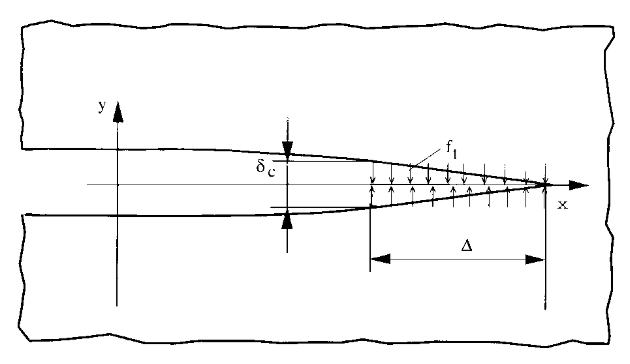
\includegraphics[width=\columnwidth]{IndependentProject/projectplan/Dougale.PNG}
    \caption{Single Crack (Dugdale) Model. \cite{Abu15}}
    \label{fig:dugdale}
\end{figure}

\bigbreak
The single crack model in Fig. \ref{fig:dugdale} assumes a crack tip located in a fracture process zone (\texttt{FPZ}). Plastic bonding stress $\sigma\leq f_{\rm{t}}$ causes the crack tip to open up, up to a critical separation length $\delta=\delta_{\rm{c}}$ \cite{Abu15}. 

\bigbreak
To determine the bonding stress, the \texttt{Y} code adopts the \texttt{Mohr-Coulomb} constitutive model \cite{Lat15}, described by

\begin{equation}
    \label{eq:MohrCoulomb}
    \tau=c+\sigma\,{\rm{tan}}\phi\,,
\end{equation}

with shear stress $\tau$, normal stress $\sigma$, internal cohesion $c$ and internal friction angle $\phi$. The internal friction coefficient is given by

\begin{equation}
    \label{eq:intfriccoeff}
    \eta={\rm{tan}}\phi
\end{equation}

The stresses $\sigma$ and $\tau$ correspond to normal and shear displacements $\delta_{\rm{n}}$ and $\delta_{\rm{s}}$ and tensile and shear strengths $f_{\rm{t}}$ and $f_{\rm{s}}$. These material strengths are defined as the maximum strength in the stress-displacement diagram (Fig. \ref{fig:FractureEnergy}), with maximum elastic displacement $\delta_{\rm{p}}$ and critical displacement $\delta_{\rm{s}}$.

\begin{figure}[!htbp]
    \centering
    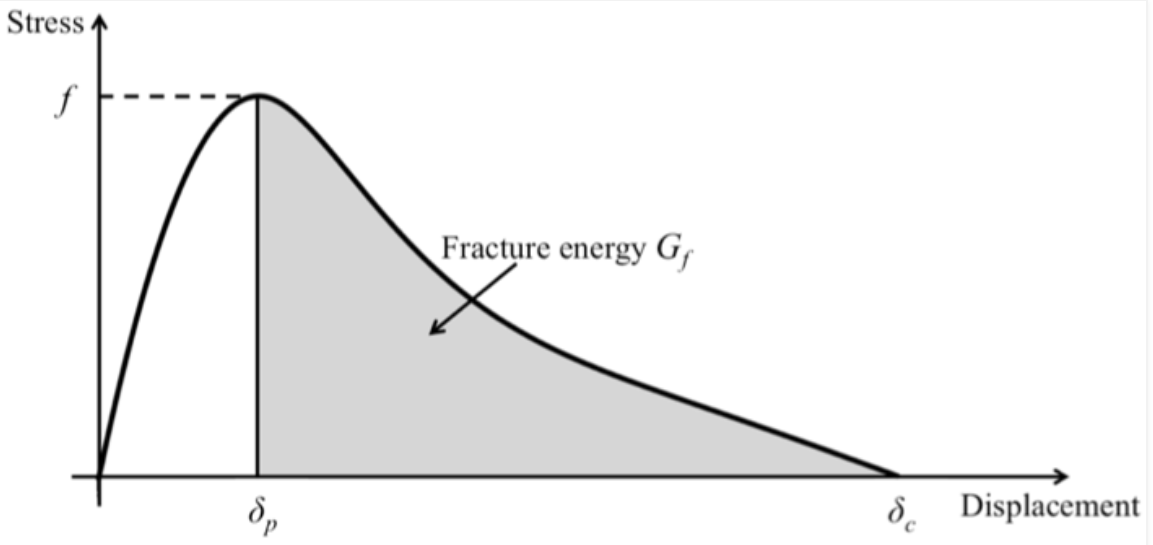
\includegraphics[width=\columnwidth]{FractureEnergy}
    \caption{Stress-displacement curve according to the single and smeared crack model. \cite{Lat15}}
    \label{fig:FractureEnergy}
\end{figure}

The fracturing in the strain-softening part is modelled using joint elements which are generated between two neighbouring shell elements. Cracks coincide with the element edges \cite{Abu15}.

\bigbreak
Further description is given for instance by Latham et al \cite{Lat15}, Munjiza et al \cite{Mun04}, Lei et al \cite{Lei16} and Chen and Chang \cite{Che18}.

\subsection{Inter-layer Model}

The task of the inter-layer is the absorption of impact energy and the maintenance of adhesion to the plies \cite{Wu14}. The inter-layer consists of one or more sheets. Common inter-layer materials include polymers such as polyvinyl butyral (\texttt{PVB}), thermoplastic polyurethane (\texttt{TPU}), and most recently \texttt{SentryGlas}\textregistered Plus (\texttt{SGP}) \cite{Moh18, Wan18}. 

\bigbreak
Mechanical properties of the inter-layer are dependent on the fracture state of the laminated glass \cite{Kun15}. Prior to fracture, straining of the inter-layer is limited, permitting the application of linear visco-elastic laws. After the failure of the glass, the inter-layer is subject to large strains and linear visco-elasticity is no longer applicable. Instead, the inter-layer is modelled as a hyper-elastic material \cite{Gha15, Kim15}. Work done by stresses onto such materials only depends on the reference state $X$ and the current state $x$, but not on the load path (Fig. \ref{fig:deformation}). Deformation from $X$ to $x$ is described by a deformation gradient \cite{Gu07}

\begin{equation}
    \label{eq:defgrad}
    F = \frac{{\rm{d}}\varphi}{{\rm{d}}X}
\end{equation}

with mapping function $\varphi$ mapping from $X$ to $x$.

\begin{figure}[!htbp]
    \centering
    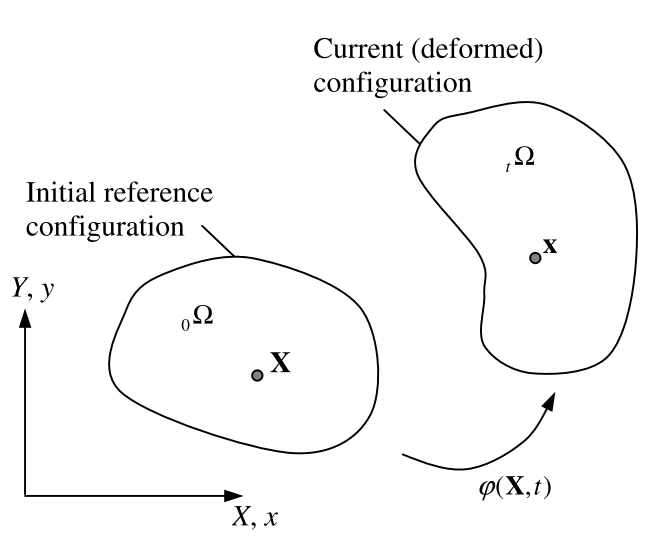
\includegraphics[width=\columnwidth]{Deformation}
    \caption{Deformation from reference to current state. \cite{Gu07}}
    \label{fig:deformation}
\end{figure}

Hyper-elastics are mathematically described by a characteristic strain energy density function $W$. One of the simplest hyper-elastic models is the \texttt{Neo-Hookean} model \cite{Gha15} whose characteristic function is given by

\begin{equation}
    \label{eq:NeoHooke}
    W=\frac{\mu_{\rm{0}}}{2}\left(I_{\rm{1}}-3\right)-\mu_{\rm{0}}\,{\rm{ln}}\,J+\frac{\lambda_{\rm{0}}}{2}{\rm{ln}}^2\,J\,,
\end{equation}

with Lam\'{e} constants $\lambda_{\rm{0}}$ and $\mu_{\rm{0}}$ from the linearised theory, $J=\lvert F\rvert$ and first invariant $I_{\rm 1}=C_{\rm{II}}$ with right Cauchy stress tensor \cite{Gha15}

\begin{equation}
    C_{\rm{ij}}=F_{\rm{Ii}}\,F_{\rm{Ij}}\,.
\end{equation}

Upper case indices refer to the reference configuration, while lower case indices refer to the current configuration.

\bigbreak
Another common, simple hyper-elastic model is the \texttt{Mooney - Rivlin} model \cite{Aba13, Kum16}. The characteristic strain energy function for the compressible 2-Parameter \texttt{Mooney - Rivlin} model \cite{Kum16} is given by

\begin{equation}
    \label{eq:MooneyRivlinSEF}
    W_{\rm{2}} = C_{\rm{10}}\left(\bar{I}_{\rm{1}}-1\right)+C_{\rm{01}}\left(\bar{I}_{\rm{2}}-1\right)+\frac{1}{d}\,(J-1)\,,
\end{equation}

where $C_{\rm{10}}$ and $C_{\rm{01}}$ are adjustable parameters, $d=2\,/\,K$ with bulk modulus $K$ and $\bar{I}_{\rm{1}}=J^{-\frac{1}{3}}\,I_{\rm{1}}$ and $\bar{I}_{\rm{2}}=J^{-\frac{1}{3}}\,I_{\rm{2}}$ are deviatoric invariants \cite{Aba13}. The second invariant is given by

\begin{equation}
    I_{\rm{2}}=\frac{1}{2}\left(C^2_{JJ}-C_{IK}C_{KI}\right)\,.
\end{equation}

\bigbreak
Other hyper-elastic models \cite{Aba13} include a more general polynomial model, \texttt{Arruda-Boyce}, \texttt{Ogden} and \texttt{Yeoh}. For the polynomial model, customized coefficients \cite{Sam19} already exist in the literature, specifically for laminated glass.

\bigbreak
Modelling the occurence of fracture needs to be permitted for the inter-layer as well, as fracturing of the inter-layer is possible. This consideration necessitates the extension of the smeared single and combined fracture model to the inter-layer.